\documentclass[11pt,a4paper]{article}

\usepackage[T1]{fontenc}
\usepackage[utf8]{inputenc}
\usepackage{lmodern}
\usepackage{microtype}
\usepackage[a4paper,margin=2.5cm]{geometry}
\usepackage{amsmath,amssymb}
\usepackage{booktabs}
\usepackage{graphicx}
\usepackage{tikz}
\usepackage{xcolor}
\usepackage[colorlinks=true,linkcolor=accent,citecolor=accent,urlcolor=accent]{hyperref}
\definecolor{accent}{HTML}{B4532A}

\title{\textbf{The Visual \LaTeX{} Workbench}}
\author{TeXPro Demo}
\date{\today}

\begin{document}
\maketitle

\begin{abstract}
This document is a live demo for TeXPro. It is ordinary, portable \LaTeX{}: every
visual element you see in the editor still compiles with \texttt{pdflatex}. Click a
rendered equation to reveal its source, then click away to render it again.
\end{abstract}

\section{Writing without leaving the page}

Visual editors usually ask authors to choose between a pretty surface and a
trustworthy source. TeXPro keeps both. Inline mathematics such as
$e^{i\pi}+1=0$ and $\langle \psi | \hat{H} | \psi \rangle$ is rendered in place,
while section headings, emphasis, tables, and figures adopt their final shape.
The source remains the document of record.

\begin{equation}
  \label{eq:energy}
  E = mc^2 + \frac{1}{2}mv^2
\end{equation}

Equation~\eqref{eq:energy} is a real numbered equation. Cross-references are
collected from the project, and \texttt{latexmk} resolves them on compile.

\subsection{A quiet writing surface}

Focus mode dims everything except the current paragraph. Typewriter mode keeps
the caret at a stable vertical position, so the page moves instead of your eyes.
Neither mode changes the file.

\begin{align}
  \nabla \cdot \mathbf{E} &= \frac{\rho}{\varepsilon_0}, \\
  \nabla \times \mathbf{B} &= \mu_0\mathbf{J}
    + \mu_0\varepsilon_0\frac{\partial \mathbf{E}}{\partial t}.
\end{align}

\section{Project-aware typesetting}

\subsection{Tables that look like tables}

The table below is rendered from its \texttt{tabular} source while the cursor is
elsewhere. Put the cursor inside it to edit the cells.

\begin{table}[h]
  \centering
  \begin{tabular}{lrr}
    \toprule
    Engine & First run (s) & Warm run (s) \\
    \midrule
    pdfLaTeX & 1.8 & 0.9 \\
    XeLaTeX  & 2.4 & 1.2 \\
    LuaLaTeX & 2.1 & 1.1 \\
    \bottomrule
  \end{tabular}
  \caption{A small benchmark table.}
  \label{tab:bench}
\end{table}

\subsection{Figures and citations}

Figure~\ref{fig:curve} is included with the standard \texttt{graphicx} package.
The editor resolves the path relative to the project and previews the image.

\begin{figure}[h]
  \centering
  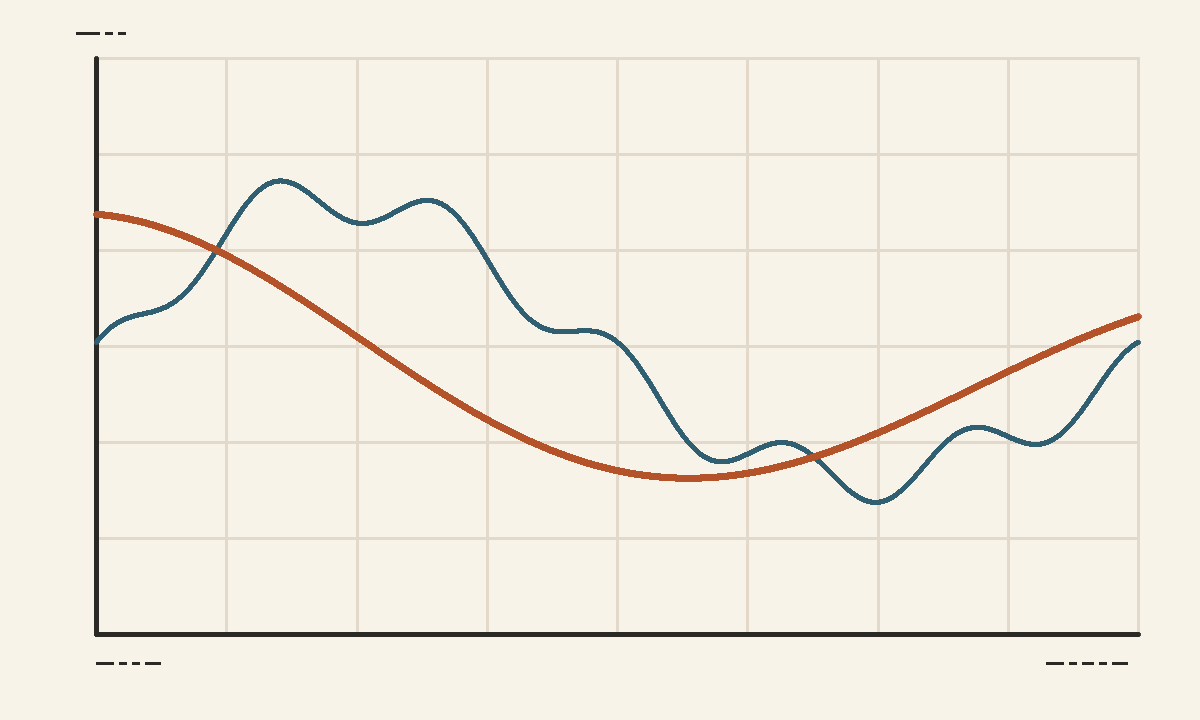
\includegraphics[width=0.78\linewidth]{assets/curve.png}
  \caption{A generated curve, previewed inline and in the PDF.}
  \label{fig:curve}
\end{figure}

Good typesetting systems separate content from presentation
\cite{knuth1984}. The bibliography below is deliberately simple, so this demo
compiles on a stock TeX Live installation.

\section{Diagrams that stay editable}

TikZ is not treated as an opaque image. The source below is compiled in a
standalone document using this project's preamble, rendered to a crisp image,
and shown in place. Click the diagram to edit it, or open TikZ Studio for a larger canvas.

\begin{tikzpicture}[scale=1.05]
  \draw[->] (-0.2,0) -- (4.4,0) node[right] {$x$};
  \draw[->] (0,-0.2) -- (0,3.2) node[above] {$y$};
  \draw[thick,blue,domain=0:4,smooth,samples=80]
    plot (\x,{0.55*\x + 0.35*sin(2*\x r)});
  \filldraw[orange] (2,1.36) circle (2pt) node[above right] {$P$};
\end{tikzpicture}

\section{What to try}

\begin{itemize}
  \item Press \texttt{Cmd+B} to compile and watch the PDF refresh.
  \item Click the PDF while holding \texttt{Cmd} to jump back to source.
  \item Press \texttt{Cmd+K} for the command palette.
  \item Type \verb|\ref{| or \verb|\cite{| to see project-aware completion.
  \item Toggle \emph{Source} in the title bar to see the exact file.
\end{itemize}

% TODO: Try editing this comment. It appears in the outline as a task.
% The structure panel also lists sections, labels, and equations.

\begin{thebibliography}{9}
\bibitem{knuth1984}
  Donald E. Knuth.
  \newblock \emph{The \TeX{}book}.
  \newblock Addison-Wesley, 1984.
\end{thebibliography}

\end{document}
